% ============================================================================
% LaTeX Figure Templates for RS-DRL Process Diagrams
% ============================================================================
% 
% This file contains standardized figure templates organized according to
% the recommended order for thesis chapter presentation.
%
% Organization principle: Start broad → progressively refine → close the loop
%
% Note: Diagrams are currently available as PNG/SVG. Convert to PDF for
% optimal LaTeX integration. File paths assume a 'figures/' subdirectory.
%
% ============================================================================

% ----------------------------------------------------------------------------
% PREAMBLE (Add to your main LaTeX document preamble)
% ----------------------------------------------------------------------------
% Required packages:
% \usepackage{graphicx}
% \usepackage{float}
% \usepackage{caption}
%
% Optional but recommended caption setup:
% \captionsetup{
%     font=small,
%     labelfont=bf
% }

% ============================================================================
% FIGURE TEMPLATES (Organized in Recommended Order)
% ============================================================================

% ----------------------------------------------------------------------------
% Figure 1 — Diagram Map (Navigation Figure)
% Purpose: Orient the reader, show abstraction layers, provide roadmap
% Source file: diagram-map.puml → diagram-map.png/svg
% ----------------------------------------------------------------------------
\begin{figure}[t]
    \centering
    \adjustbox{width=0.95\textwidth,height=0.85\textheight,center,keepaspectratio}{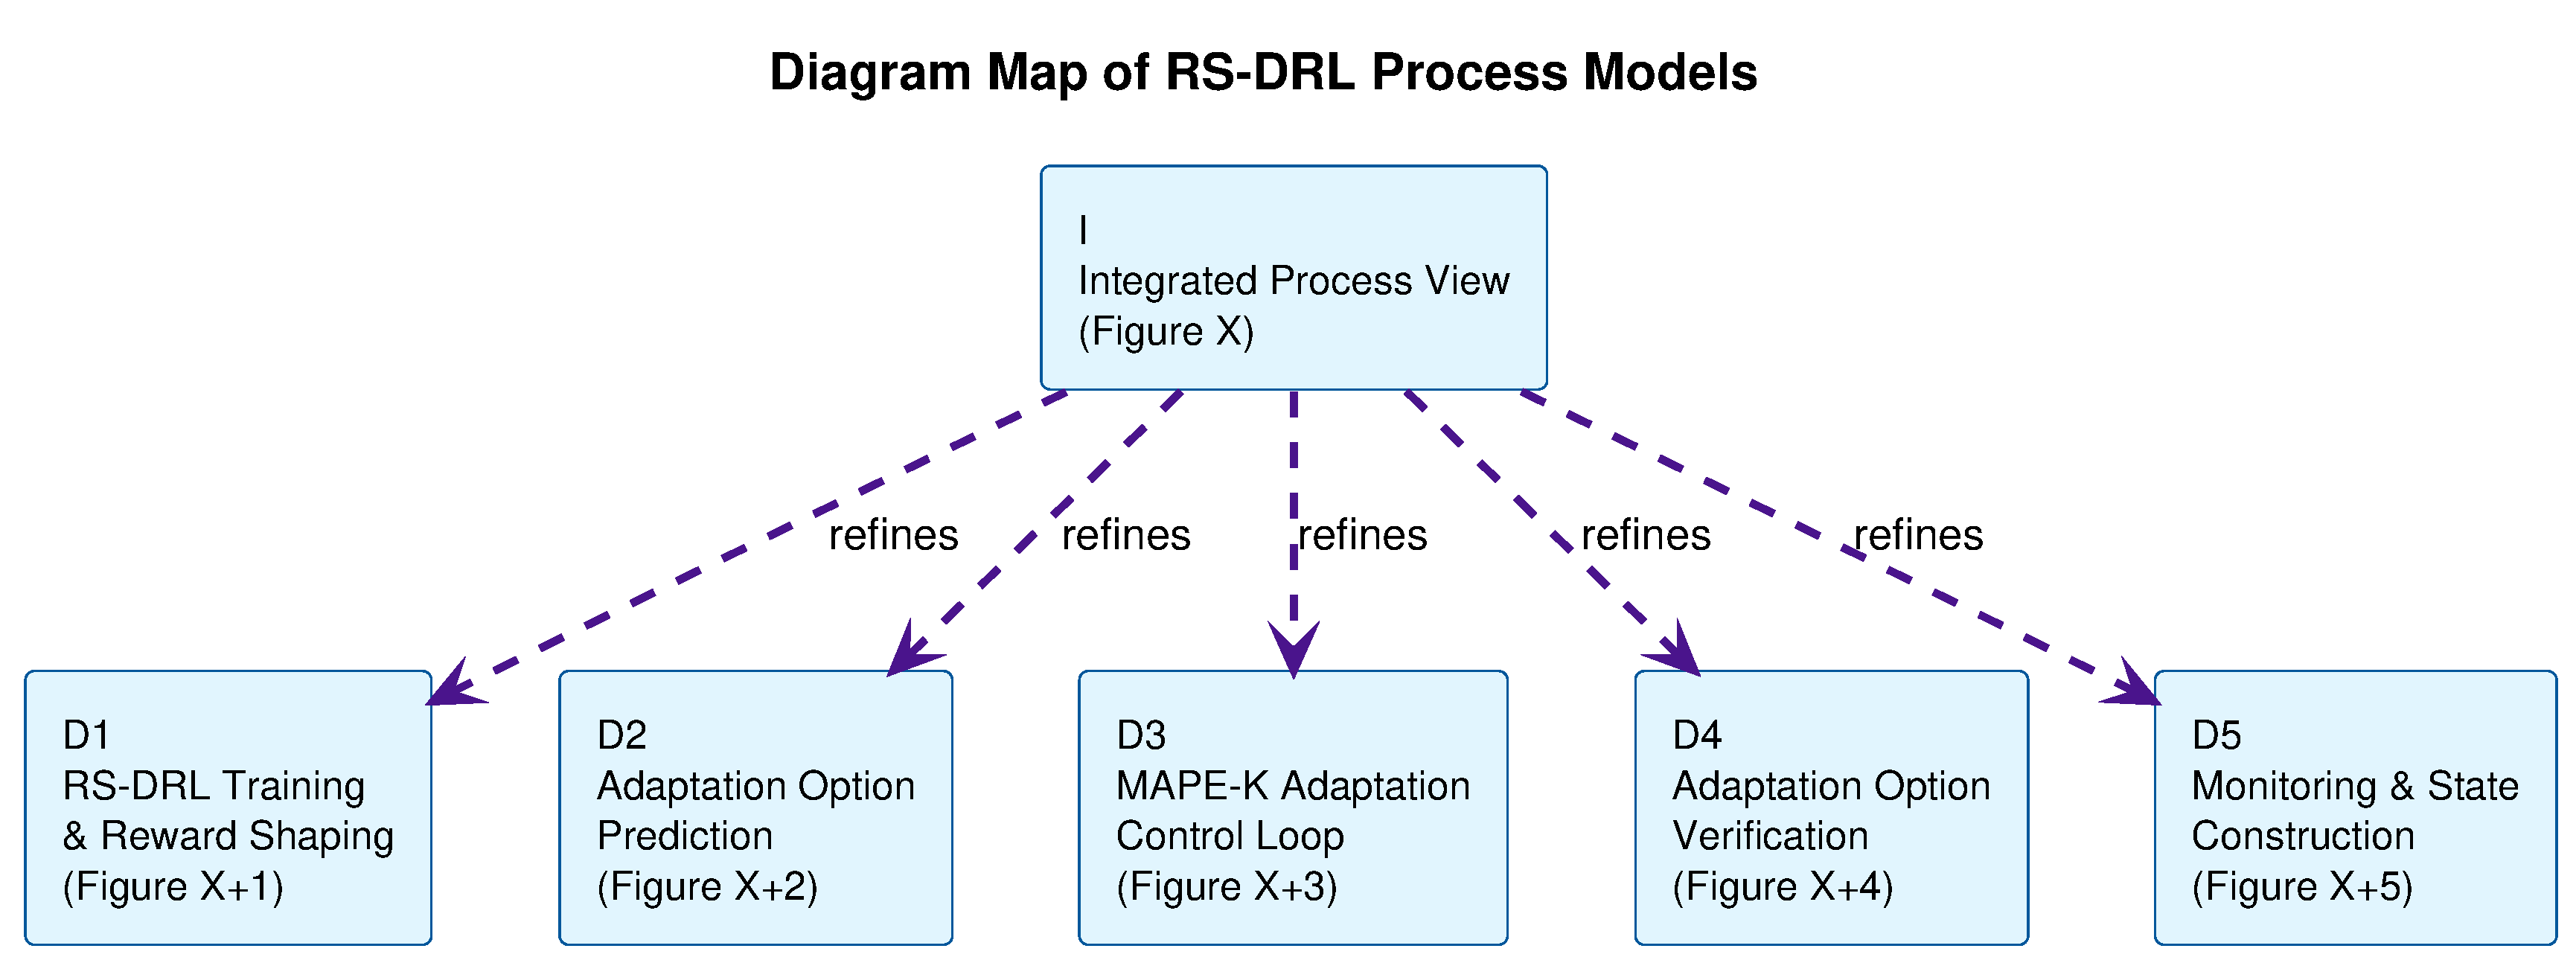
\includegraphics{figures/diagram-map-rs-drl.pdf}}
    \caption{Diagram map of the RS-DRL-based self-adaptive system. 
    The central integration diagram provides a high-level process view, 
    while Diagrams D1--D5 refine the learning, decision-making, verification, control, 
    and monitoring subprocesses presented in this chapter.}
    \label{fig:diagram-map}
\end{figure}

% ----------------------------------------------------------------------------
% Figure 2 — High-Level Integration Process Overview
% Purpose: Show the 9 numbered integration stages as a sequential flow
% Source file: rs-drl-integration-overview.puml → rs-drl-integration-overview.png/svg
% ----------------------------------------------------------------------------
\begin{figure}[t]
    \centering
    \adjustbox{width=0.95\textwidth,height=0.85\textheight,center,keepaspectratio}{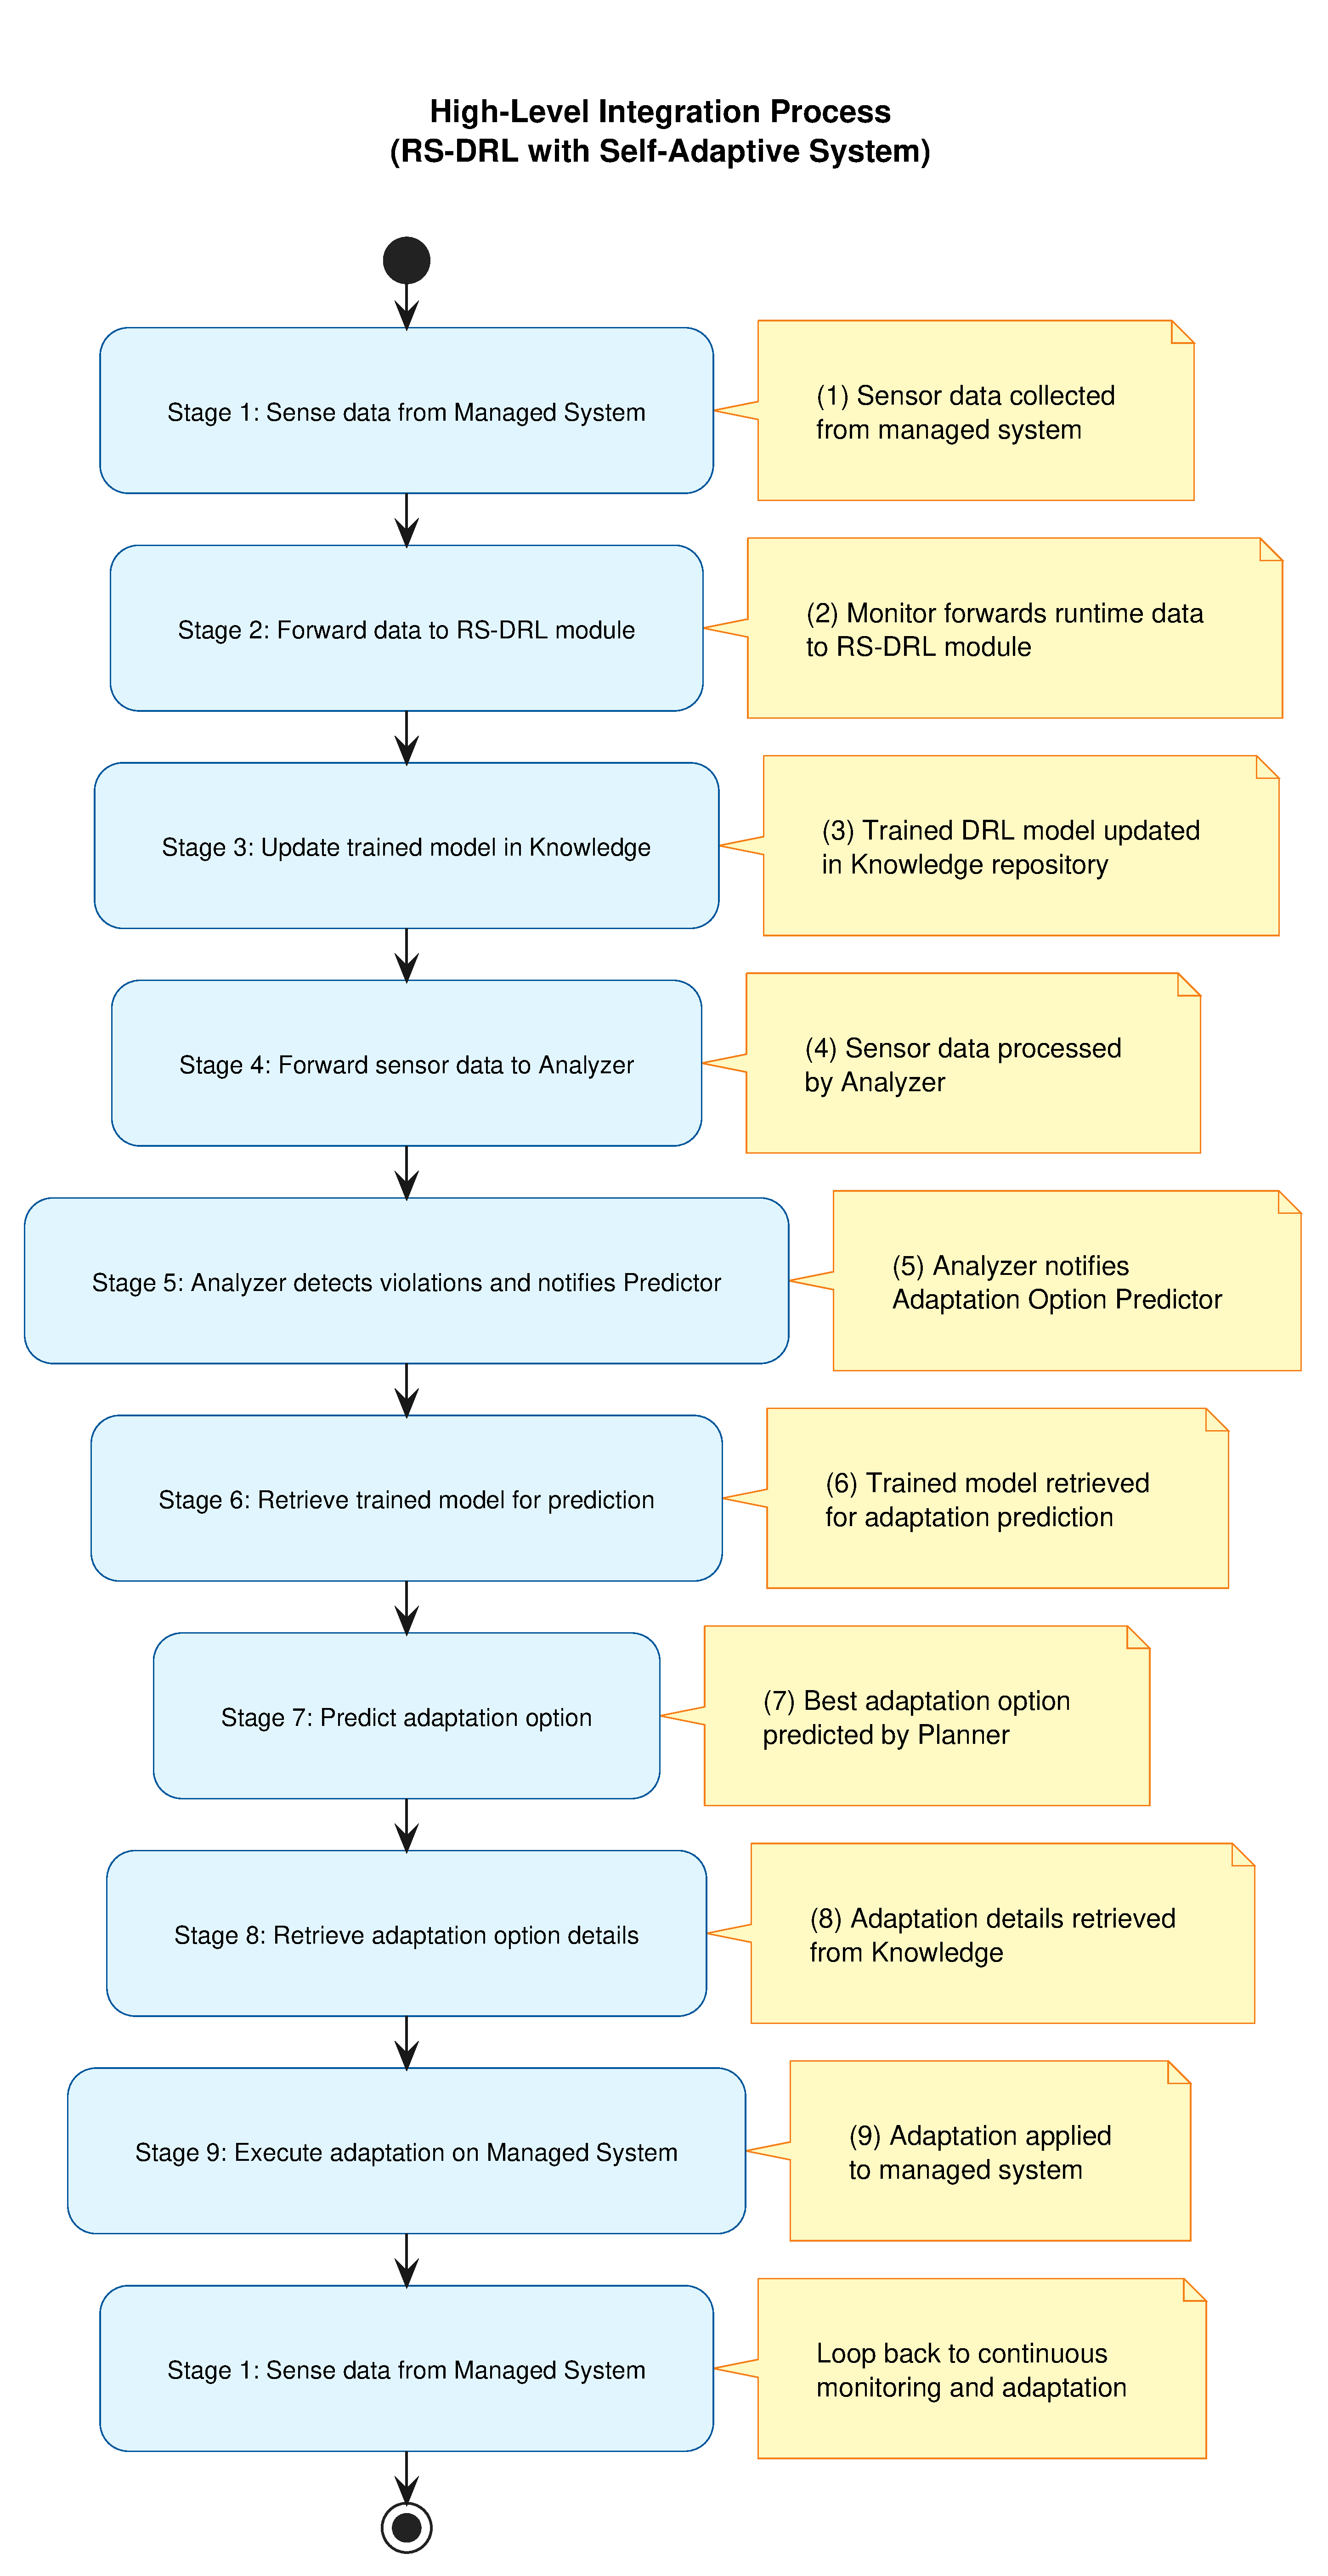
\includegraphics{figures/rs-drl-integration-overview.pdf}}
    \caption{High-level integration process overview showing the nine numbered stages 
    of the RS-DRL-based self-adaptive system. The sequential flow illustrates how 
    data sensing, feature extraction, model updates, analysis, planning, and execution 
    are integrated in a continuous adaptation loop.}
    \label{fig:integration-overview}
\end{figure}

% ----------------------------------------------------------------------------
% Figure 3 — Integrated Process View
% Purpose: Show full closed-loop behavior, explain system orchestration
% Source file: rs-drl-integrated-system.puml → rs-drl-integrated-system.png/svg
% ----------------------------------------------------------------------------
\begin{figure}[t]
    \centering
    \adjustbox{width=0.95\textwidth,height=0.85\textheight,center,keepaspectratio}{\includegraphics{figures/integrated-process-view.pdf}}
    \caption{Integrated process view of the RS-DRL-based self-adaptive system. 
    The figure illustrates the closed-loop interaction between monitoring, learning, 
    verification, planning, and execution, and refines the original architectural view 
    presented in Figure~4 of the reference model.}
    \label{fig:integration}
\end{figure}

% ----------------------------------------------------------------------------
% Figure 4 — Monitoring & State Construction (Diagram 5)
% Purpose: First detailed refinement - show how raw data becomes state vector
% Source file: monitoring-state-construction.puml → monitoring-state-construction.png/svg
% ----------------------------------------------------------------------------
\begin{figure}[t]
    \centering
    \adjustbox{width=0.9\textwidth,height=0.85\textheight,center,keepaspectratio}{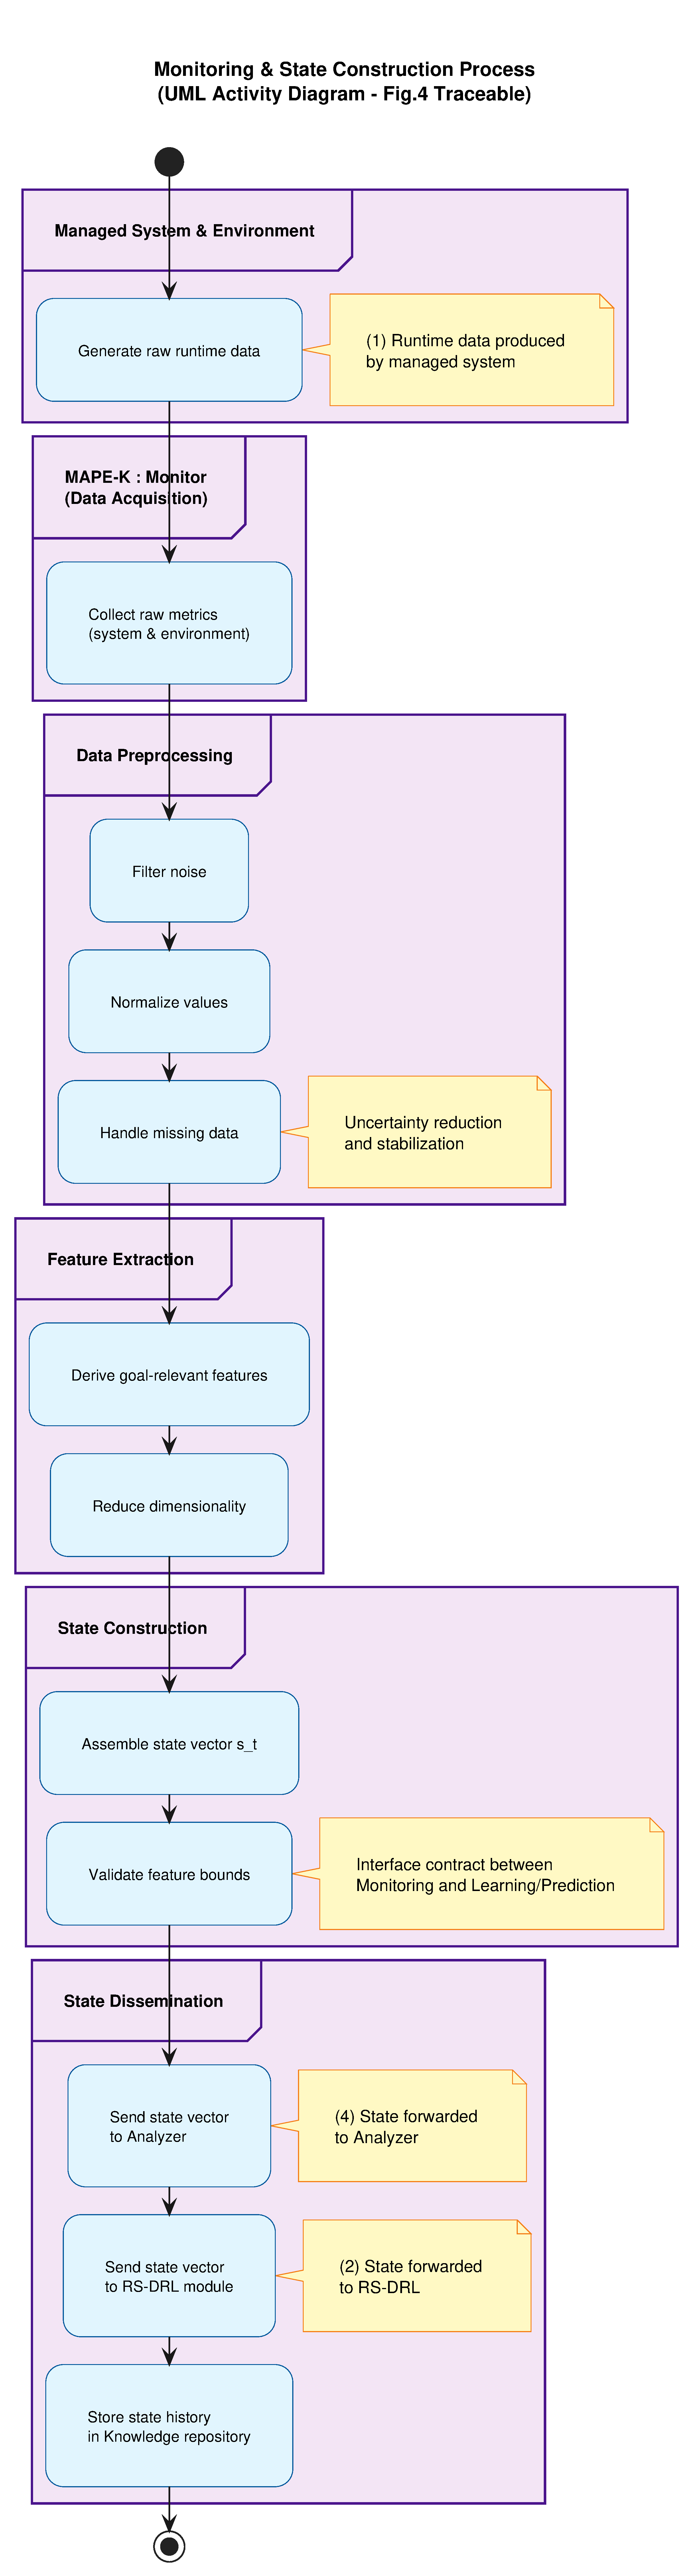
\includegraphics{figures/monitoring-state-construction.pdf}}
    \caption{Monitoring and state construction process. 
    Raw runtime data from the managed system and environment is filtered, 
    abstracted, and transformed into a state vector suitable for both 
    RS-DRL learning and runtime adaptation analysis.}
    \label{fig:monitoring}
\end{figure}

% ----------------------------------------------------------------------------
% Figure 5 — RS-DRL Training & Reward Shaping (Diagram 1)
% Purpose: Technical core - show how learning happens
% Source file: rs-drl-training-process.puml → rs-drl-training-process.png/svg
% ----------------------------------------------------------------------------
\begin{figure}[t]
    \centering
    \adjustbox{width=0.95\textwidth,height=0.85\textheight,center,keepaspectratio}{\includegraphics{figures/rs-drl-training.pdf}}
    \caption{RS-DRL training and reward shaping process. 
    The figure details the episodic interaction with the environment, 
    experience replay, and the novel reward reshaping mechanism applied 
    during minibatch learning.}
    \label{fig:training}
\end{figure}

% ----------------------------------------------------------------------------
% Figure 5a — Reward Shaping Micro-Process
% Purpose: Isolate and make explicit the novel reward shaping mechanism
% Source file: reward-shaping-process.puml → reward-shaping-process.png/svg
% ----------------------------------------------------------------------------
\begin{figure}[t]
    \centering
    \adjustbox{width=0.8\textwidth,height=0.85\textheight,center,keepaspectratio}{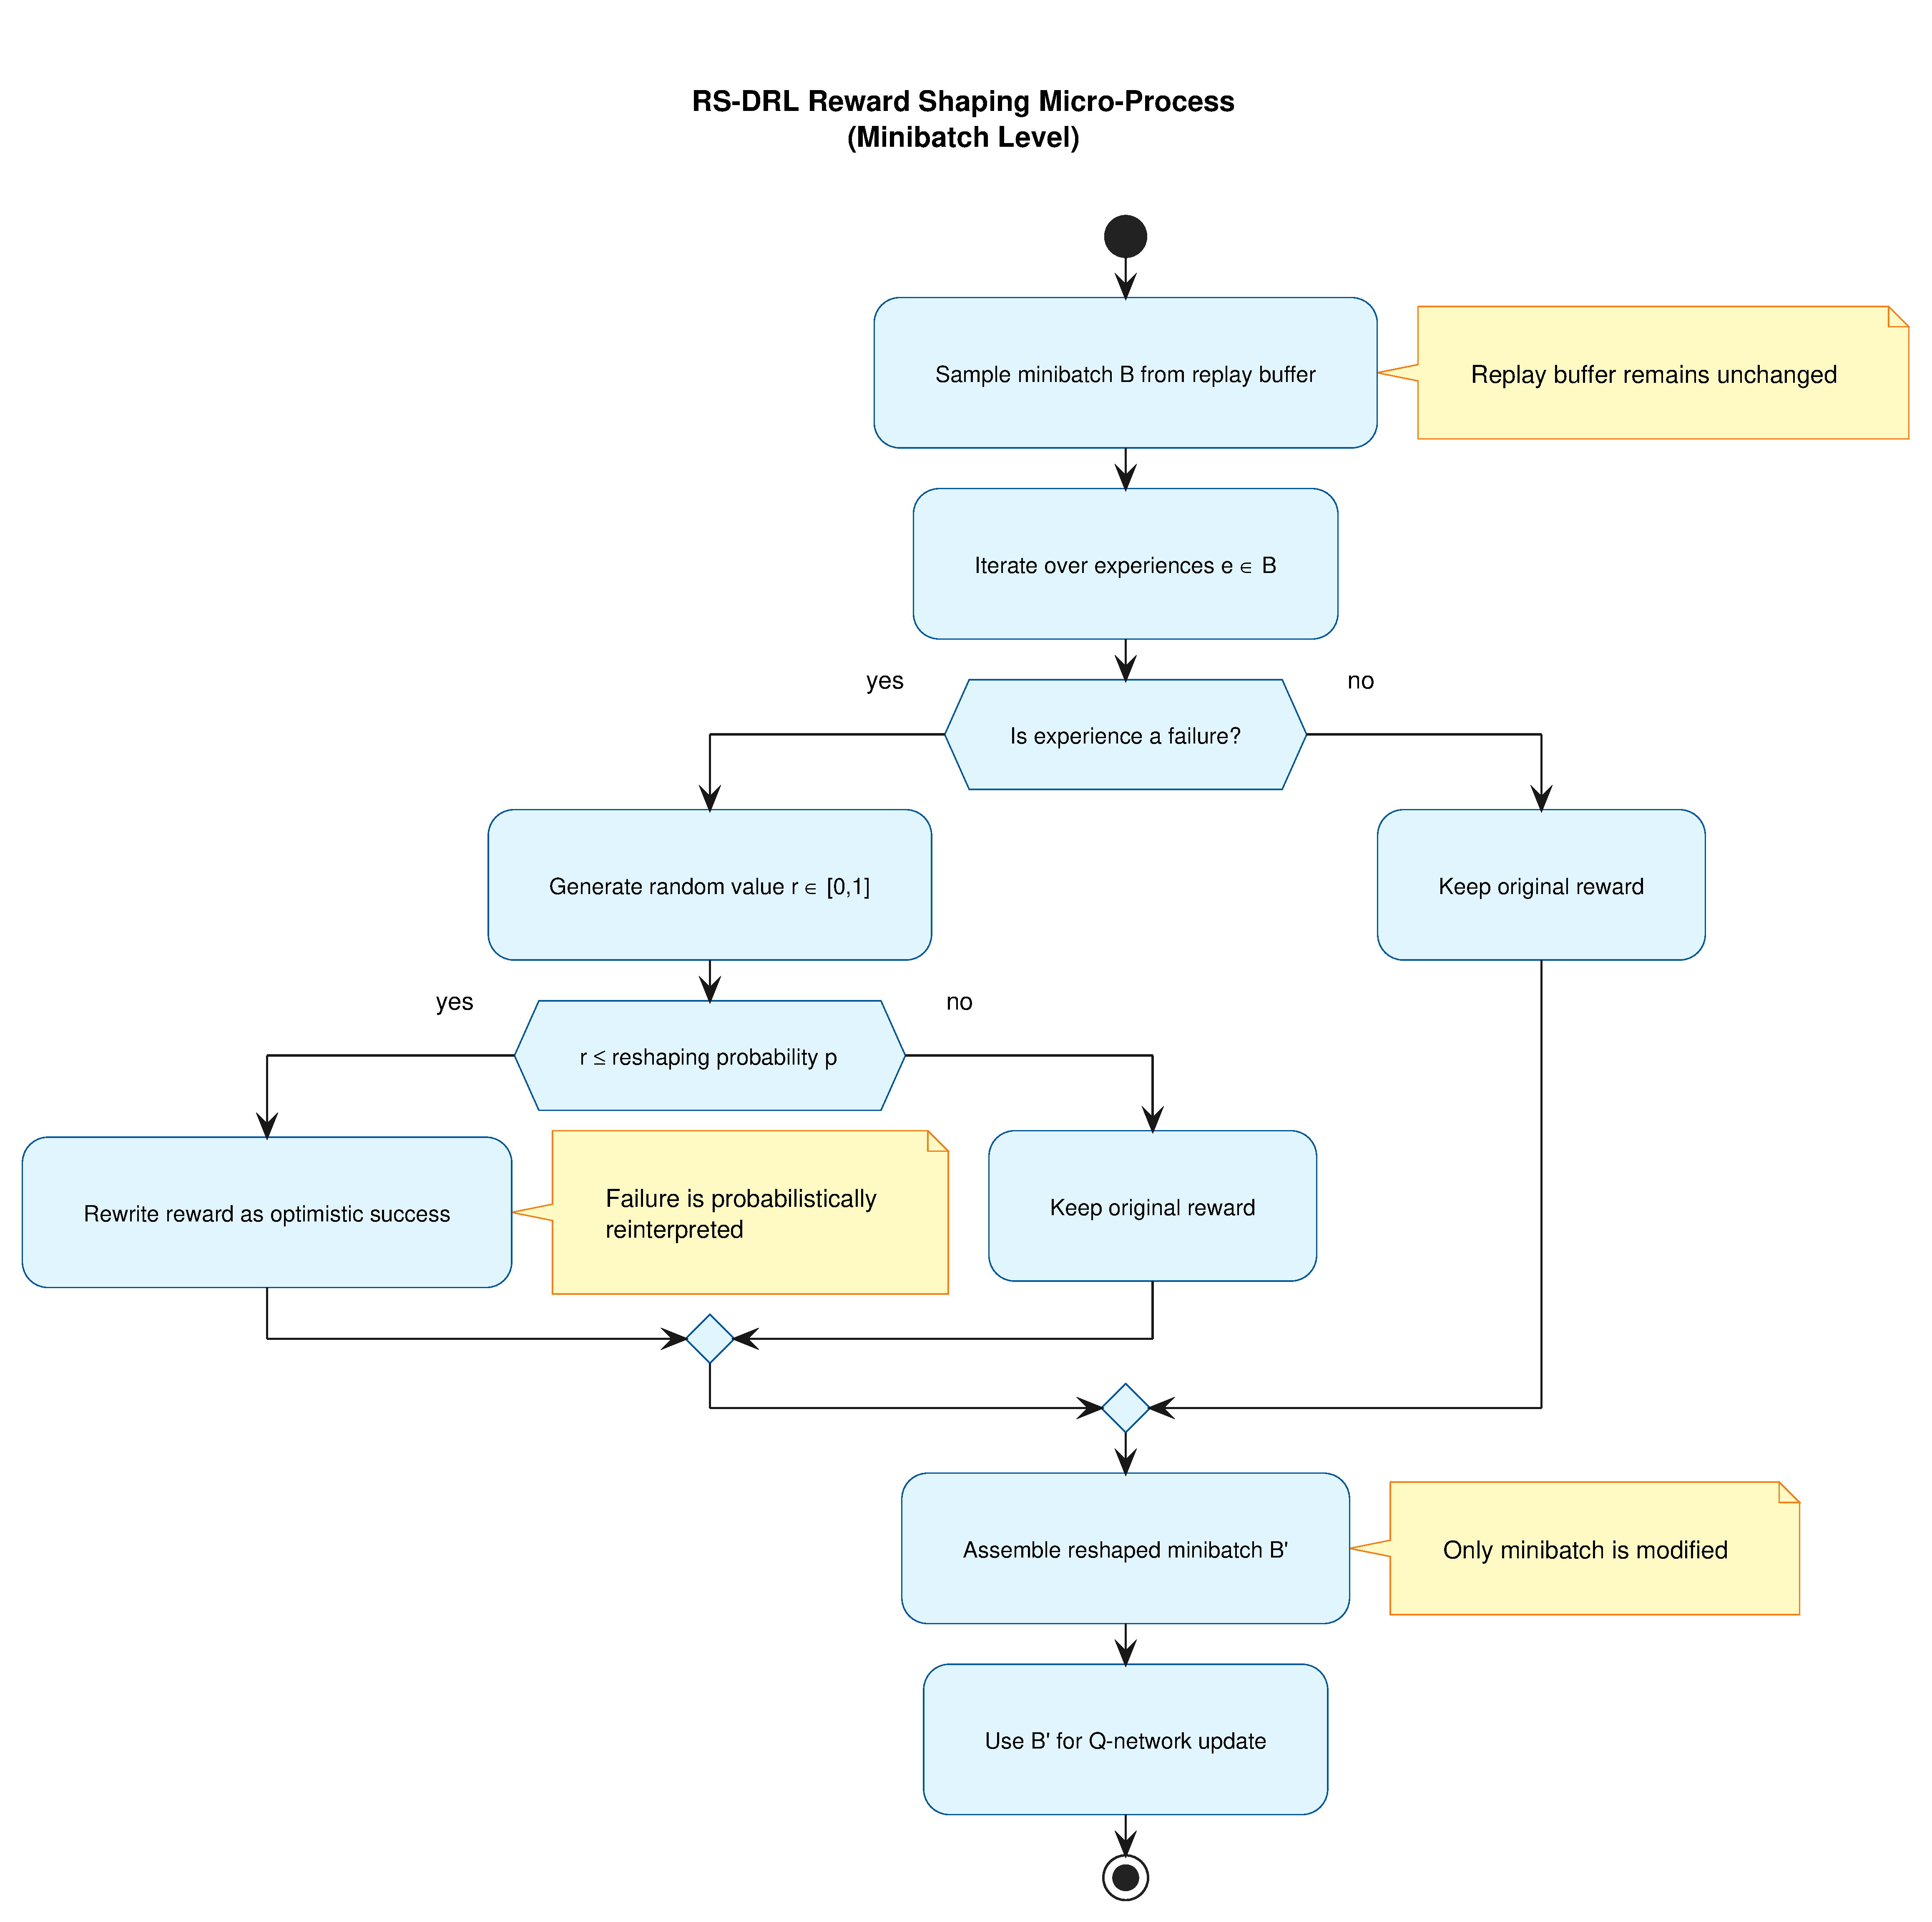
\includegraphics{figures/reward-shaping-process.pdf}}
    \caption{Reward shaping micro-process applied during RS-DRL training.
    Failed experiences sampled in a minibatch are probabilistically reinterpreted as optimistic successes
    according to a reshaping probability~$p$.
    Reward reshaping is applied exclusively to the sampled minibatch and does not modify the replay buffer,
    preserving experience diversity while accelerating learning convergence.}
    \label{fig:reward-shaping}
\end{figure}

% ----------------------------------------------------------------------------
% Figure 6 — Adaptation Option Prediction (Diagram 2)
% Purpose: Runtime intelligence - show how decisions are made
% Source file: adaptation-option-prediction.puml → adaptation-option-prediction.png/svg
% ----------------------------------------------------------------------------
\begin{figure}[t]
    \centering
    \adjustbox{width=0.8\textwidth,height=0.85\textheight,center,keepaspectratio}{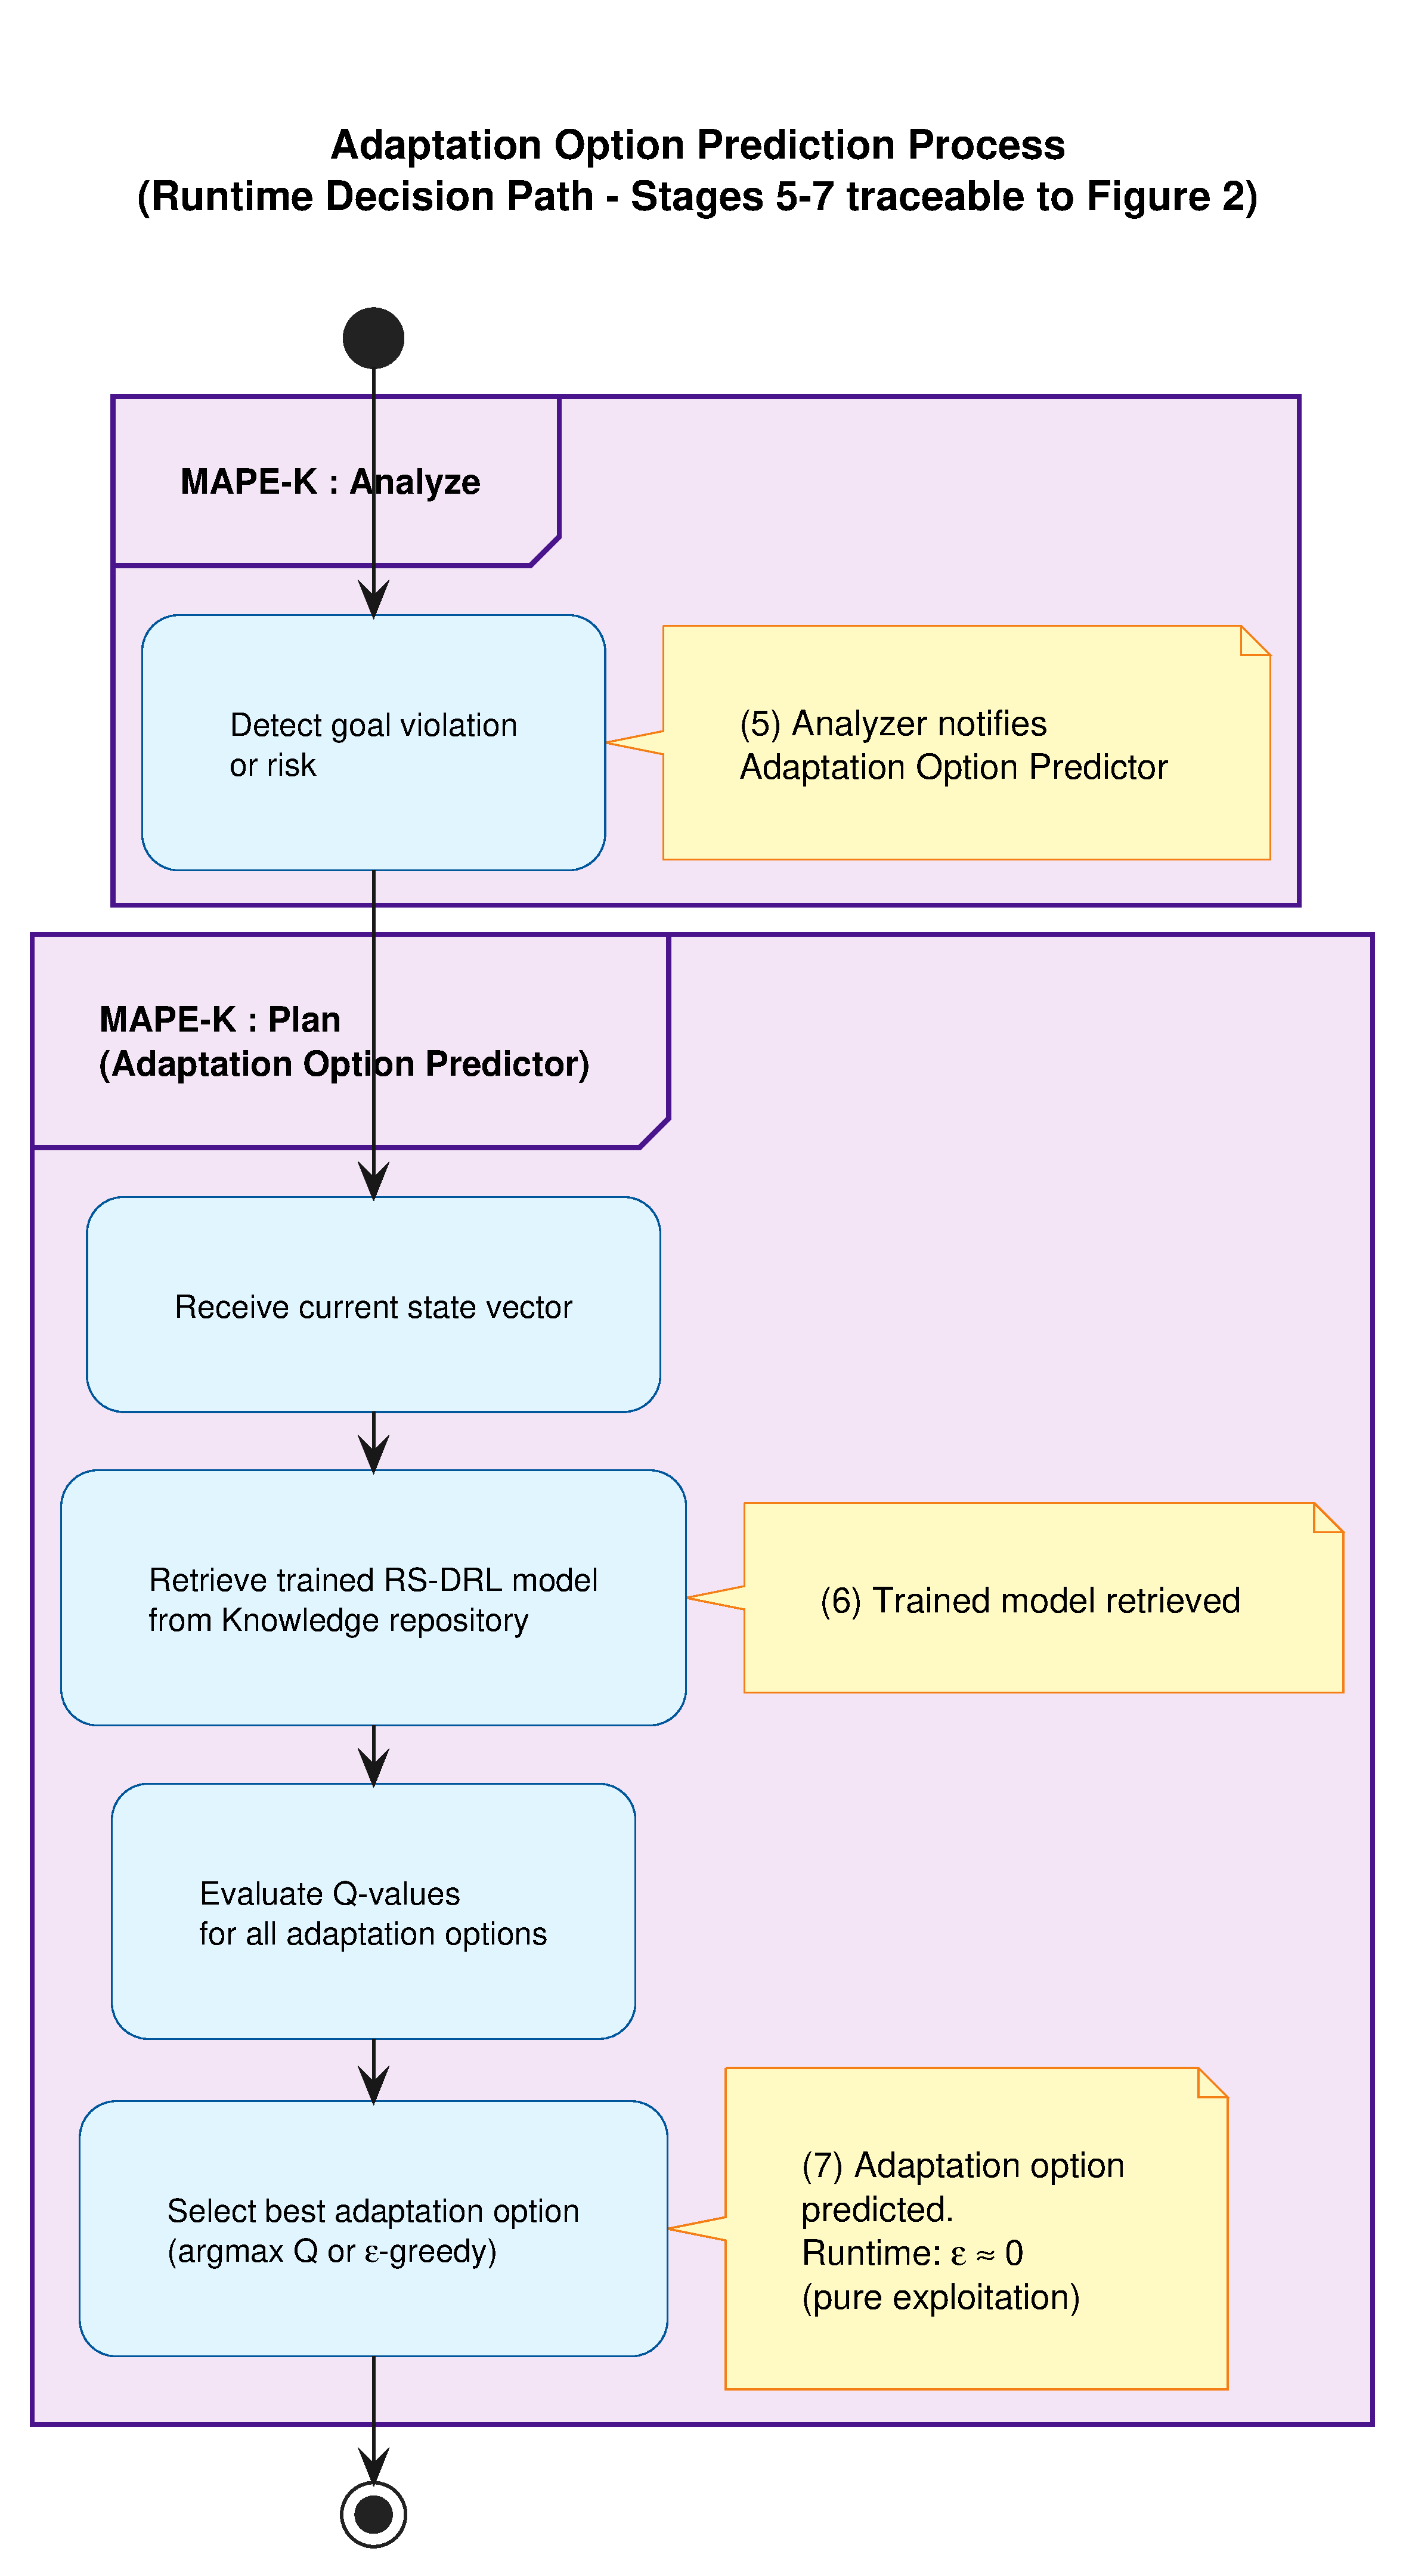
\includegraphics{figures/adaptation-prediction.pdf}}
    \caption{Adaptation option prediction process at runtime. 
    Upon detection of goal violations, the trained RS-DRL model is used 
    to predict the most suitable adaptation option without further learning.}
    \label{fig:prediction}
\end{figure}

% ----------------------------------------------------------------------------
% Figure 7 — MAPE-K Adaptation Control Loop (Diagram 3)
% Purpose: System-level coordination - show when and why adaptation happens
% Source file: mape-k-adaptation-control-loop.puml → mape-k-adaptation-control-loop.png/svg
% ----------------------------------------------------------------------------
\begin{figure}[t]
    \centering
    \adjustbox{width=0.9\textwidth,height=0.85\textheight,center,keepaspectratio}{
\includegraphics{figures/mape-k-loop.pdf}}
    \caption{MAPE-K adaptation control loop. 
    The figure illustrates how monitoring and analysis trigger adaptation, 
    how planning delegates decision making to the RS-DRL predictor, 
    and how execution enacts the selected adaptation.}
    \label{fig:mape-k}
\end{figure}

% ----------------------------------------------------------------------------
% Figure 8 — Adaptation Option Verification (Diagram 4)
% Purpose: Trust and correctness - show why decisions are trustworthy
% Source file: adaptation-option-verification.puml → adaptation-option-verification.png/svg
% ----------------------------------------------------------------------------
\begin{figure}[t]
    \centering
    \adjustbox{width=0.9\textwidth,height=0.85\textheight,center,keepaspectratio}{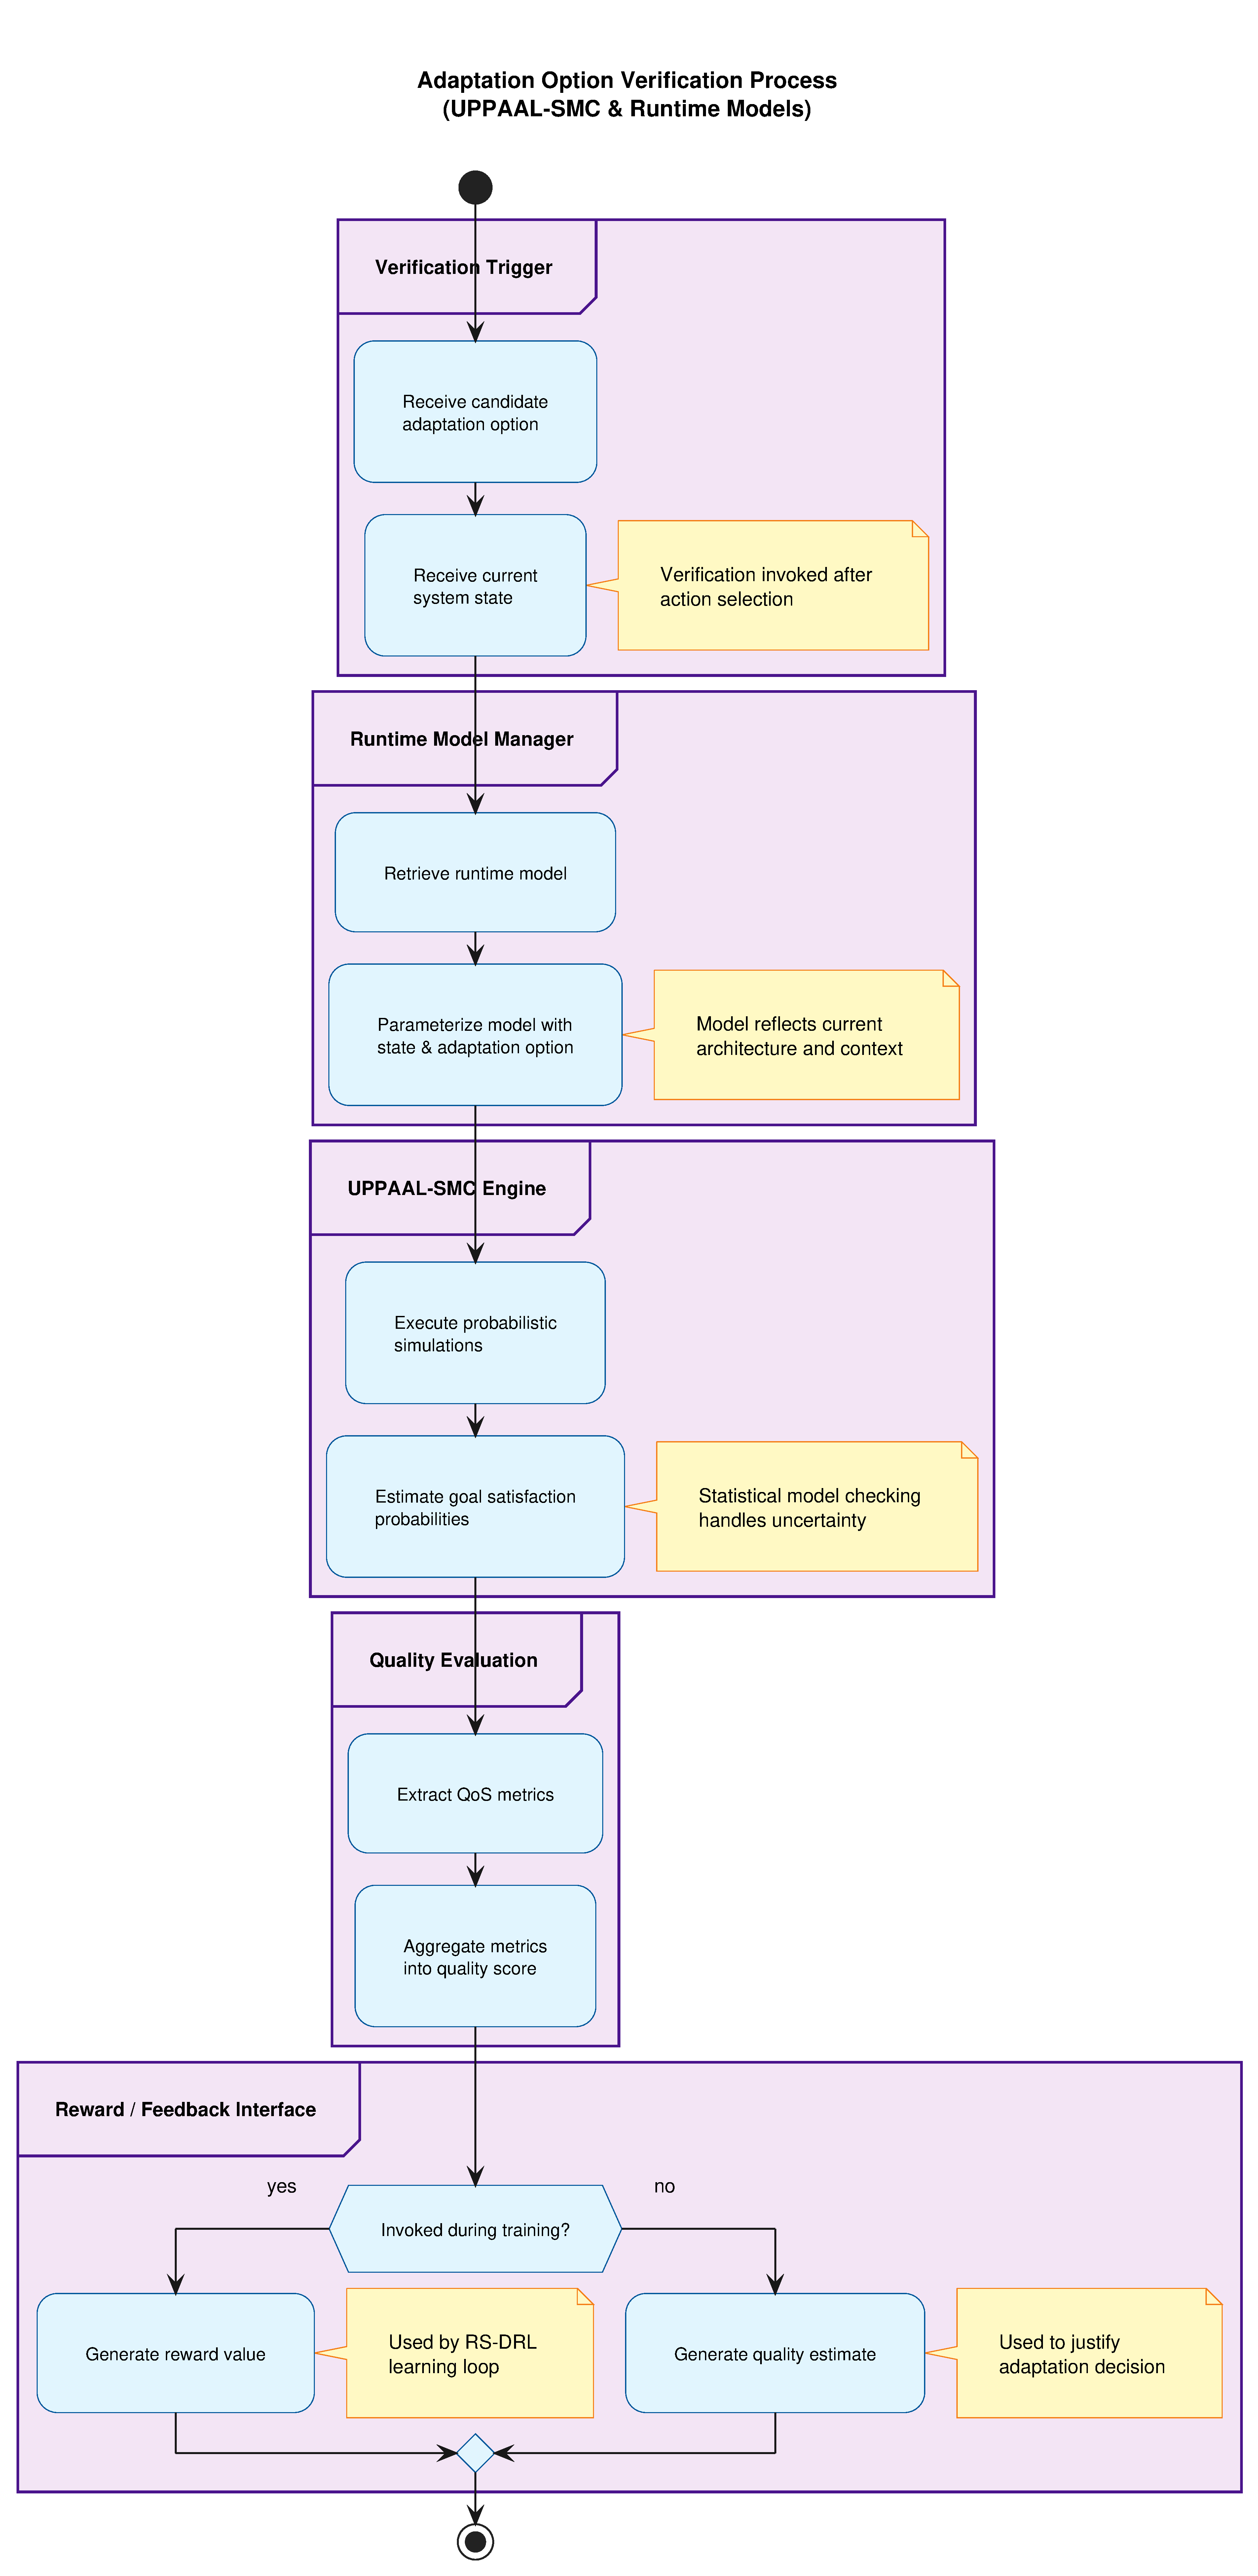
\includegraphics{figures/adaptation-verification.pdf}}
    \caption{Adaptation option verification using runtime models and statistical model checking. 
    The verification process evaluates the expected quality of adaptation options 
    under uncertainty and provides feedback for learning and decision justification.}
    \label{fig:verification}
\end{figure}

% ============================================================================
% FILE NAME MAPPING NOTES
% ============================================================================
%
% Current source files → Expected PDF filenames for LaTeX:
%
% diagram-map.*              → diagram-map-rs-drl.pdf
% rs-drl-integration-overview.* → rs-drl-integration-overview.pdf
% rs-drl-integrated-system.* → integrated-process-view.pdf
% monitoring-state-construction.* → monitoring-state-construction.pdf
% rs-drl-training-process.*  → rs-drl-training.pdf
% adaptation-option-prediction.* → adaptation-prediction.pdf
% mape-k-adaptation-control-loop.* → mape-k-loop.pdf
% adaptation-option-verification.* → adaptation-verification.pdf
%
% Note: You may need to rename files or create symbolic links to match
% the expected names in the LaTeX templates. Alternatively, update the
% file paths in this template to match your actual file names.
%
% For PDF conversion:
% - SVG files can be converted to PDF using tools like Inkscape or online converters
% - PNG files can be converted to PDF using ImageMagick or similar tools
% - For best quality, use SVG → PDF conversion
%
% ============================================================================

